%
% 2-cauchy.tex -- 2. Cauchy-Integralsatz
%
% (c) 2025 Prof Dr Andreas Müller
%
\section{Der Integralsatz
\label{buch:integration:section:cauchy}}
\kopfrechts{Der Integralsatz von Cauchy}
Das Beispiel~\ref{buch:integration:wege:bsp:kreisintegral} hat
gezeigt, dass mit Ausnahme des Falls $n=-1$ die Potenzen $z^n$ 
das Wegintegral über einen Kreis um den Nullpunkt den Wert 0
ergab.
Für $\frac{1}{z}$ ergab sich der Wert
\[
\oint_{S^1} \frac{dz}{z}
=
2\pi i.
\]
Der Homotopiebegriff erlaubt, die Wege beliebig zu deformieren,
solange der Definitionsbereich der Funktion nicht verlassen wird.
Es scheint, dass das Integral über geschlossene Wege vor allem davon
abhängt, was in Polstellen des Integranden passiert.
Der Residuensatz, der in diesem Abschnitt hergeleitet werden soll,
formalisiert diese Beobachtung.

%
% 21-geschlossen.tex -- Wegintegrale über geschlossene Wege
%
% (c) 2026 Prof Dr Andreas Müller
%
\subsection{Wegintegrale über geschlossene Wege}
%
% fig-residuum.tex
%
% (c) 2026 Prof Dr Andreas Müller
%
\begin{figure}
\centering
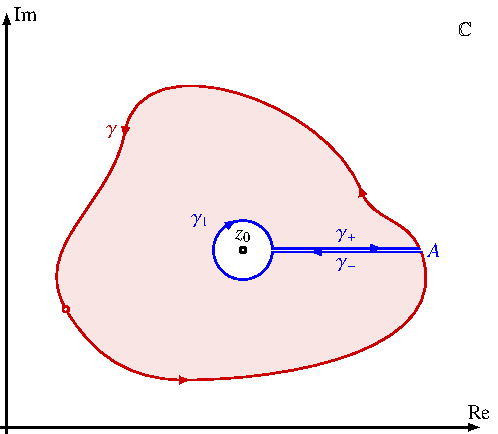
\includegraphics{chapters/030-integration/images/residuum.pdf}
\caption{Herleitung des Integralsatzes.
Der Weg $\gamma$ wird durch die Segmente $\gamma_-$, $\gamma_1$ und
$\gamma_+$ zu einem Weg ergänzt, der das hellrote Gebiet berandet,
in dem die Funktion $f(z)/(z-z_0)$ holomorph ist.
\label{buch:integration:homologie:fig:residuum}}
\end{figure}
%
Nach dem Satz~\ref{buch:integration:wegintegral:satz:zusammenziehbar}
von Abschnitt~\ref{buch:integration:wegintegral:subsection:homotopie}
verschwindet das Integral einer holomorphen Funktion entlang eines
zusammenziehbaren Weges.
Wir betrachten jetzt eine holomorphe Funktion $f$ in einem Gebiet $U$
und einen Punkt $z_0\in U$
und einen Weg $\gamma$, der den Punkt $z_0\in U$
einmal im Gegenuhrzeigersinn umläuft
(siehe Abbildung\ref{buch:integration:homologie:fig:residuum}).
Die Funktion
\[
f_0
\colon
U\setminus\{z_0\}
\to
\mathbb{C}
:
z
\mapsto
\frac{f(z)}{z-z_0}
\]
ist immer noch holomorph.
Der Weg $\gamma$ ist jetzt im Definitionsgebiet $U\setminus \{z_0\}$
der Funktion $f_0$ nicht mehr zusammenziehbar, er müsste über den Punkt
$z_0$ hinweggezogen werden, wo die Funktion $f_0$ nicht definiert ist.
Man kann also nicht erwarten, dass das Integral von $f_0(z)$ über
den Weg $\gamma$ verschwindet.
Vielmehr gilt der folgende, viel überraschendere Satz.

\begin{satz}[Cauchy]
\label{buch:integration:satz:residuensatz}
\index{Satz!Cauchy-Integralformel}%
\index{Cauchy-Integralformel}%
Sei $f\colon U\to\mathbb{C}$ holomorphe Funktion und $\gamma\colon I\to U$
ein geschlossener Weg, der den Punkt $z_0$ einmal im Gegenuhrzeigersinn
umläuft.
Dann gilt
\begin{equation}
f(z_0)
=
\frac{1}{2\pi i}
\oint_{\gamma} \frac{f(z)}{z-z_0}\,dz.
\label{buch:integration:eqn:residuensatz}
\end{equation}
\end{satz}

\begin{proof}
Die Berechnung des Integrals
\eqref{buch:integration:eqn:residuensatz}
wird dadurch erschwert, dass der Weg $\gamma$ den Punkt $z_0$
umläuft, der nicht im Definitionsgebiet liegt.
Wir ergänzen ihn daher zu einem geschlossenen Weg, der ein
ganz in $U\setminus\{z_0\}$ liegendes Gebiet berandet.
Dazu fügen wir beim Punkt $A$ die in 
Abbildung~\ref{buch:integration:homologie:fig:residuum}
blau eingezeichneten Wegstücke $\gamma_-$, $\gamma_1$ und $\gamma_+$ 
ein.
In der Zeichnung haben die Wege $\gamma_-$ und $\gamma_+$ aus Gründen
der Darstellung einen kleinen Abstand, in Wahrheit sollen diese beiden
Wegstücke bis auf die Durchlaufrichtung identisch sein.
Nach dem Homotpiesatz gilt jetzt
\begin{equation}
\int_{\gamma
\cdot
\gamma_-
\cdot
\gamma_1
\cdot
\gamma_+
}
\frac{f(z)}{z-z_0}\,dz
=
0,
\label{buch:integration:residuensatz:eqn:proof1}
\end{equation}
weil die Funktion im hellrot gefärbten Gebiet, welches vom zusammengesetzten
Weg berandet wird, holomorph ist.

Die Wegstücke $\gamma_-$ und $\gamma_+$ werden in entgegengesetzter 
Richtung durchlaufen.
Verkettet bilden sie einen zusammenziehbaren Weg im Definitionsgebiet
der der Funktion $f_0$.
Die Wegintegrale über diese beiden Teilstücke heben sich also weg.

Vom Integral auf der linken Seite von
\eqref{buch:integration:residuensatz:eqn:proof1}
bleiben jetzt nur noch die Integrale über die beiden Wegstücke
$\gamma$ und $\gamma_1$,
die sich wegen \eqref{buch:integration:residuensatz:eqn:proof1}
ebenfalls wegheben müssen.
Es gilt also
\begin{equation}
0
=
\int_{\gamma+\gamma_1}
\frac{f(z)}{z-z_0}
\,dz
=
\oint_{\gamma}
\frac{f(z)}{z-z_0}
\,dz
+
\oint_{\gamma_1}
\frac{f(z)}{z-z_0}
\,dz
\quad\Rightarrow\quad
\oint_\gamma
\frac{f(z)}{z-z_0}
\,dz
=
-
\oint_{\gamma_1}
\frac{f(z)}{z-z_0}
\,dz.
\label{buch:integration:residuensatz:eqn:proof2}
\end{equation}

Zur Berechnung des Integrals über $\gamma_1$ verwenden wir die
Parametrisierung
\[
\gamma_1
\colon
I
\to
\mathbb{C}
:
t
\mapsto
\gamma_1(t)
=
z_0
+
re^{-2\pi i t}.
\]
mit der Ableitung 
\[
\dot{\gamma}_1(t)
=
-2\pi i r e^{-2\pi it}.
\]
Damit können wir das Wegintegral über $\gamma_1$ berechnen und
erhalten
\begin{align}
\int_{\gamma_1}
\frac{f(z)}{z-z_0}\,dz
&=
\int_0^1
f_0(\gamma_1(t))\cdot \dot{\gamma}_1(t)\,dt
\\
&=
\int_0^1
\frac{f(z_0+re^{-2\pi it})}{e^{-2\pi it}}
\cdot(-2\pi i r e^{-2\pi it})
\,dt
\notag
\\
&=
-2\pi i
\int_0^1
f(z_0+re^{-2\pi it})
\,dt.
\notag
\intertext{Nach dem Homotpiesatz~\ref{buch:integration:satz:homotopie} 
bleibt das letzte Integral gleich, wenn der Radius $r$ des kleinen
Kreises $\gamma_1$ verkleinert wird.
Insbesondere gilt im Grenzübergang $r\to 0$}
\int_{\gamma_1}
\frac{f(z)}{z-z_0}\,dz
&=
\lim_{r\to 0}
\biggl(
-2\pi i
\int_0^1
f(z_0+re^{-2\pi it})
\,dt
\biggr)
\notag
\\
&=
-2\pi i
\int_0^1
f(z_0)\,dt
=
-2\pi if(z_0).
\label{buch:integration:residuensatz:eqn:proof3}
\end{align}
Indem man das Resultat
\eqref{buch:integration:residuensatz:eqn:proof3}
in
\eqref{buch:integration:residuensatz:eqn:proof2}
einsetzt, findet man jetzt
\[
\oint_\gamma
\frac{f(z)}{z-z_0}
\,dz
=
2\pi if(z_0)
\qquad\Rightarrow\qquad
f(z_0)
=
\frac{1}{2\pi i}
\oint_\gamma
\frac{f(z)}{z-z_0}
\,dz.
\]
Damit ist der Satz bewiesen.
\end{proof}

Der Satz sagt, dass die Werte der holomoprhen Funktion $f(z)$ im
Inneren des Weges vollständig durch die Werte der Funktion auf
dem Weg $\gamma$ bestimmt sind.

%
% 22-pole.tex -- Wegintegrale und Pole
%
% (c) 2026 Prof Dr Andreas Müller
%
\subsection{Wegintegrale und harmonische Funktionen}
Sei $f\colon U\to\mathbb{C}$ eine holomorphe Funktion und
$a\in U$ ein Punkt.
Sei weiter $\gamma$ ein geschlossener Weg, der den Punkt $a$
einmal im Gegenuhrzeigersinn umkreist.

%
% Mittelwerteigenschaft
%
\subsubsection{Mittelwerteigenschaft}
Aus der Formel~\eqref{buch:integration:eqn:residuensatz} folgt auch
sofort die folgende Eigenschaft einer harmonischen Funktion.

\begin{satz}[Mittelwerteigenschaft]
\label{buch:integration:cauchy:satz:mittelwerteigenschaft}
\index{Mittelwerteigenschaft}%
Sei $U\subset\mathbb{C}$ ein Gebiet und $z_0\in U$ ein Punkt in $U$.
Weiter sei $u$ eine harmonische Funktion in $U$ und $r$ der Radius
eines Kreises um den Punkt $z_0$, der immer noch ganz in $U$ enhalten ist.
Dann ist
\begin{equation}
u(z_0)
=
\frac{1}{2\pi}
\int_0^{2\pi} u(z_0 + re^{it}) \,dt.
\label{buch:integration:cauchy:eqn:mittelwerteigenschaft}
\end{equation}
\end{satz}

\begin{proof}
Zunächst kann nach Satz~\ref{buch:holomorph:holomorph:satz:utov}
eine Funktion $v$ gefunden werden, so dass in einer Umgebung, die auch
den Kreis mit Radius $r$ um $z_0$ enthält, $f(z) = u(z) + iv(z)$ eine
holomorphe Funktion ist.
Nach dem Residuensatz ist dann
\[
f(z_0)
=
\frac{1}{2\pi i}
\oint_{S^1_r(z_0)} 
\frac{f(z)}{z-z_0}
\,dz
\]
für den Kreis $S^1_r(z_0)$ mit Radius $r$ um den Punkt $z_0$.
Den Weg kann man durch $t\mapsto z_0+e^{it}$ parametrisieren,
dann wird das Integral zu
\begin{align*}
f(z_0)
&=
\frac{1}{2\pi i}
\int_0^{2\pi}
\frac{ f(z_0+re^{it}) }{z_0+re^{it}-z_0} ir e^{it}\,dt
=
\frac{1}{2\pi}
\int_0^{2\pi}
\frac{ f(z_0+re^{it}) }{re^{it}} r e^{it}\,dt
\\
&=
\frac{1}{2\pi}
\int_0^{2\pi}
 f(z_0+re^{it})\,dt.
\intertext{Den Integranden kann man in Real- und Imaginärteil aufspalten und
erhält}
u(z) + iv(z)
&=
\frac{1}{2\pi}
\int_0^{2\pi}
u(z_0+re^{it})\,dt
+
\frac{i}{2\pi}
\int_0^{2\pi}
v(z_0+re^{it})\,dt.
\end{align*}
Die Formel~\eqref{buch:integration:cauchy:eqn:mittelwerteigenschaft}
gilt daher sowohl für $u$ wie auch für $v$ ganz unabhängig von der
Wahl der Funktion $v$.
\end{proof}

%
% Maximumprinzip
%
\subsubsection{Maximumprinzip}
Aus der Mittelwerteigenschaft folgt eine weitere wichtige Eigenschaft
harmonischer Funktionen, nämlich das Maximum- und Minimum-Prinzip.

\begin{satz}[Maximumprinzip]
\index{Maximumprinzip}%
Sei $U\subset\mathbb{C}$ ein Gebiet und $u(x,y)$ eine in $U$ harmonische
Funktion.
Dann nimmt die Funktion $u$ ihr Maximum und Minimum auf dem Rand von $U$ an.
\end{satz}

\begin{proof}
Wir zeigen, dass das Maximum oder Minimum nicht im Inneren des Gebietes
$U$ liegen kann.
Dazu nehmen wir an, das Maximum liegt im Punkt $z_0\in U$.
Sei $r>0$ der Radius eines Kreises um den Punkt $z_0$, der vollständig
in $U$ enthalten ist.
Dann ist $u(z_0+ re^{i\varphi}) < u(z_0)$ für alle Winkel $\varphi$,
die Werte auf dem Kreis sind kleiner als der Wert im Punkt $z_0$.
Da die Werte auf dem Kreis kleiner sind als der Wert $u(z_0)$,
ist der Mittelwert $<u(z_0)$.
Nach Satz~\ref{buch:integration:cauchy:satz:mittelwerteigenschaft} ist
der Mittelwert der Werte auf dem Kreis mit Radius $r$ um $z_0$ gleich dem
Wert $u(z_0)$, ein Widerspruch.
Der Widerspruch zeigt, dass $z_0$ nicht ein Maximum sein kann.

Auf die gleiche Weise kann man den Fall eines Minimums behandeln.
\end{proof}

Das Maximumprinzip gilt für die Lösungen einer homogenen partiellen
Differentialgleichung mit einem beliebigen elliptischen Operator.
Der Beweis folgt allerdings einem ganz anderen Weg, denn die
Mittelwerteigenschaft gilt für solche Lösungen nicht.
Für eine ausführliche Diskussion siehe \cite[section 6.4]{buch:evans}.

%
% 23-ableitungen.tex -- Ableitungen
%
% (c) 2026 Prof Dr Andreas Müller
%
\subsection{Ableitungen}
Der Satz~\ref{buch:integration:satz:residuensatz} zeigt, wie der
Wert einer holomorphen Funktion in einem Punkt $z_0$ allein aus den
Werten entlang eines Weges berechnet werden kann, der den Punkt $z_0$
im Gegenuhrzeigersinn umläuft.
Die durch die Formel
\eqref{buch:integration:eqn:residuensatz}
gegebene Funktion ist holomorph, man sollte daher auch die Ableitung
mit Hilfe eines Integrals berechnen können.
Wenn man 
\eqref{buch:integration:eqn:residuensatz}
unter dem Integral nach $z_0$ ableitet, erhält man
\begin{align}
f'(z_0)
=
\frac{d}{dz_0}f(z_0)
&=
\frac{1}{2\pi i}
\oint_{\gamma}
\frac{d}{dz_0}
\frac{f(z)}{z-z_0}
\,dz
\notag
\\
&=
\frac{1}{2\pi i}
\oint_{\gamma}
\frac{f(z)}{(z-z_0)^2}
\,dz.
\label{buch:integration:eqn:ableitung2}
\end{align}
Wie erwartet kann die Ableitung von $f$ ebenfalls durch ein einfaches
Wegintegral berechnet werden.
Durch wiederholtes Ableiten kann man auch höhere Ableitungen finden,
wie der folgende Satz zeigt.

\begin{satz}[Cauchy-Formel für Ableitungen]
\label{buch:integration:satz:ableitungn}
\index{Satz!Cauchy-Formel für Ableitungen}%
\index{Cauchy-Ableitungsformel}%
Ist $f\colon U\to\mathbb{C}$ eine holomorphe Funktion und $\gamma$
ein Weg, der den Punkt $z_0\in U$ im Gegenuhrzeigersinn umläuft.
Dann gilt
\begin{equation}
\frac{d^n}{dz_0^n}f(z_0)
=
f^{(n)}(z_0)
=
\frac{n!}{2\pi i}
\oint_{\gamma}
\frac{f(z)}{(z-z_0)^{n+1}}
\,dz.
\label{buch:integration:eqn:ableitungn}
\end{equation}
\end{satz}

\begin{proof}
Der Fall $n=1$ ist bereits durch \eqref{buch:integration:eqn:ableitung2}
bewiesen, wir müssen die Formel
\eqref{buch:integration:eqn:ableitungn}
für $n>1$ beweisen.
Wir tun dies mit Hilfe vollständiger Induktion, wobei 
\eqref{buch:integration:eqn:ableitung2} als Induktionsverankerung
dient.

Wir nehmen jetzt an \eqref{buch:integration:eqn:ableitungn} für $n$ gilt,
und zeigen, dass sie dann auch für $n+1$ gilt.
Dazu leiten wir \eqref{buch:integration:eqn:ableitungn} nach $z_0$
ab und erhalten
\begin{align*}
f^{(n+1)}(z_0)
&=
\frac{d}{dz_0}
f^{(n)}(z_0)
=
\frac{d}{dz_0}
\frac{n!}{2\pi i}
\oint
\frac{f(z)}{(z-z_0)^{n+1}}
\,dz
\\
&=
\frac{n!}{2\pi i}
\oint
\frac{d}{dz_0}
\frac{f(z)}{(z-z_0)^{n+1}}
\,dz
\\
&=
\frac{n!}{2\pi i}
\oint
(-(n+1))
\frac{f(z)}{(z-z_0)^{n+2}}
(-1)
\,dz
\\
&=
\frac{(n+1)!}{2\pi i}
\oint
\frac{f(z)}{(z-z_0)^{n+2}}
\,dz.
\end{align*}
Damit ist \eqref{buch:integration:eqn:ableitungn} bewiesen.
\end{proof}

Die Werte und alle Ableitungen einer holomorphen Funktion in der Umgebung
eines Punktes können also durch Berechnung von Integralen der Form
\eqref{buch:integration:eqn:ableitungn}
über einen Weg, der die Umgebung umschliesst, berechnet werden.
Da der Integrand entlang des Weges stetig ist, sind diese Integrale
alle wohldefiniert.
Da das Bild des Weges kompakt ist, sind die Integrale als Funktionen
von $z_0$ stetig.
Wir erhalten damit das folgende überraschende Resultat.

\begin{korollar}
Eine holomorphe Funktion $f\colon U\to\mathbb{C}$ ist beliebig oft stetig
differenzierbar.
\end{korollar}

Einmalige komplexe Differenzierbarkeit hat also automatisch beliebige
stetige Differenzierbarkeit zur Folge.
Dies steht in krassem Gegensatz zur Situation reeller Funktionen,
wo Beispiele von einmal stetig differenzierbaren Funktionen konstruiert
worden sind, die nicht beliebig oft differenzierbar sind.
Die komplexe Differenzierbarkeit ist also eine sehr viel stärkere
Einschränkung als reelle Differenzierbarkeit.


%
% 24-liouville.tex -- Der Satz von Liouville
%
% (c) 2026 Prof Dr Andreas Müller
%
\subsection{Der Satz von Liouville}
Die Cauchy-Formel für die Ableitungen hat die unerwartete Konsquenz,
dass auf ganz $\mathbb{C}$ definierte holomorphe Funktionen, die nicht
Polynome sind, exponentiell schnell anwachsen müssen, wenn $z$ gross wird.

\begin{definition}[polynomiell beschränkt]
Eine in ganz $\mathbb{C}$ definierte komplexe Funktion $f(z)$ heisst
\emph{polynomiell beschränkt}, wenn es $N\in\mathbb{N}$ und $a>0$
\index{polynomiell beschränkt}%
gibt derart, dass
\begin{equation}
|f(z)|
\le a(1+|z|^N)
\label{buch:integration:eqn:liouvilleschranke}
\end{equation}
für alle $z\in\mathbb{C}$ gilt.
\end{definition}

\begin{satz}[Liouville]
\label{buch:integration:satz:liouville}
\index{Satz!von Liouville}%
\index{Liouville, Joseph}%
Sei $f$ eine auf ganz $\mathbb{C}$ holomorphe Funktion, die polynomiell
beschränkt ist.
Dann ist $f$ ein Polynom vom Grad höchstens $N$.
\end{satz}

\begin{proof}
Wir wenden den Satz
\ref{buch:integration:satz:ableitungn}
für Ableitungen einer holomorphen Funktion auf den Weg
$\gamma(t)=z_0+Re^{2\pi it}$.
Nach der Formel \eqref{buch:integration:eqn:ableitungn}
gilt für für alle $k$
\begin{align*}
f^{(k)}(z_0)
&=
\frac{k!}{2\pi i}
\oint_\gamma
\frac{f(z)}{(z-z_0)^{k+1}}
\,dz.
\intertext{Mit der Voraussetzung
\eqref{buch:integration:eqn:liouvilleschranke}
wir dies durch}
|f^{(k)}(z_0)|
&=
\frac{k!}{2\pi}
\oint_\gamma
\biggl|
\frac{f(z)}{(z-z_0)^{k+1}}
\biggr|
\,dz
\\
&\le
\frac{k!}{2\pi}
\int_0^1
\frac{|f(\gamma(t))|}{R^{k+1}}
2\pi R
\,dt
\\
&\le
k!
\int_0^1
\frac{|f(\gamma(t))|}{R^k}
\,dt
\\
&\le
\frac{k!}{R^k}
\int_0^1
a(1+|\gamma(t)|^N)
\,dt
\\
&\le
\frac{k!}{R^k}
\int_0^1
a(1+(|z_0|+R)^N)
\,dt
\\
&\le
k!
a
\frac{
1+(|z_0|+R)^N
}{R^k}
\end{align*}
abgeschätzt.
Für $R\to\infty$ strebt der Bruch auf der rechten Seite für $k>N$ 
gegen $0$, so dass $f^{(k)}(z_0)=0$ folgt.
Alle Ableitungen höherer als $N$-ter Ordnung der Funktion $f$ verschwinden,
also ist $f$ ein Polynom vom Grad höchstens $N$.
\end{proof}

Man beachte, dass der Grenzübergang im letzten Schritt des Beweises 
verwendet, dass die Funktion auf ganz $\mathbb{C}$ holomorph ist.
Sobald es Punkte in $\mathbb{C}$ gibt, in denen die Funktion nicht
holomorph ist, gilt auch die Integralformel nicht mehr und damit
bricht die Abschätzungskette des Beweises zusammen.

Der Spezialfall $N=0$ liefert die folgende Aussage.

\begin{korollar}
Eine beschränkte, auf ganz $\mathbb{C}$ holomorphe Funktion ist
konstant.
\end{korollar}

Für reelle Funktionen kann ein solches Resultat nicht gelten.
Die trigonometrischen Funktionen $\sin x$ und $\cos x$ sind
für alle reellen Argumente von $x$ beschränkt.
In $\mathbb{R}$ gilt für beide Funktionen
\[
|f(x)| \le 1,
\]
was der Ungleichung
\eqref{buch:integration:eqn:liouvilleschranke}
mit $N=0$ und $a=1$ entspricht.
Die trigonometrischen Funktionen sind aber alles andere als konstant
und auch keine Polynome, da Ableitungen beliebig hoher Ordnung nicht
verschwinden.

Umgekehrt bedeutet der Satz von Liouville, dass eine Funktion,
die durch eine für alle $z\in\mathbb{C}$ konvergente Potenzreihe
definiert ist, die kein Polynom ist, nicht polynomiell beschränkt
sein kann.
Für die Sinus- und Kosinusfunktionen zeigt die Definition
\[
\cos z = \frac{e^{iz}+e^{-iz}}{2}
\qquad\text{und}\qquad
\sin z = \frac{e^{z}-e^{-iz}}{2i},
\]
dass sich die Funktionen für imaginäre Argumente wie Exponentialfunktionen
verhalten, die nicht polynomiell beschränkt sind.

Holomorphe Funktionen, die keine Polynome sind, aber für grosse $z$
nur polynomiell anwachsen, können nicht in ganz $\mathbb{C}$
holomorph sein.
Rationale Funktionen, bei denen der Nennergrad grösser ist als der
Zählergrad, sind Beispiele für dieses Phänomen.
Tatsächlich hat eine solche Funktion immer mindestens eine Polstelle,
in der die Funktion nicht definiert ist.



